%% FullCourse_10Lecs -- Lecture 7, Topic 7.3a: How LLMs Work (Pretrain, Generate, Fine-tune)
%% Source: ./archive_pre_split/Lec07_LLM.tex (section 7)
%% Pass B: layer in refinements from
%%         ../../MiniCourse_8hr/Slides/Module3_LLM_Text/M3_T3a_How_LLMs_Work.tex
%%         (RLHF/DPO + scaling laws)

%% Shared preamble for the FullCourse_10Lecs topic decks.
%%
%% Each topic .tex \input's this file, then defines its own \title, \date
%% override (if any), \graphicspath, and \begin{document}.
%%
%% Reconstructed verbatim from the inlined copy preserved in
%% Lec10_Case_Studies/Lec10_T8_Case6_DeepRamsey.tex (lines 23-190), which is
%% explicitly annotated there as "from ../shared_preamble.tex, copied verbatim".
%% Base preamble matches MiniCourse_8hr/Slides/shared_preamble.tex; this version
%% additionally provides \sectiondivider, the conceptbox/cautionbox/examplebox/
%% takeawaybox tcolorboxes, and \compacttables used across the split decks.

\documentclass[10pt,english,aspectratio=169]{beamer}

\usepackage{ae,aecompl}
\usepackage[T1]{fontenc}
\usepackage{textcomp}
\usepackage[utf8]{inputenc}
\usepackage{babel}
\usepackage{datetime2}

\setcounter{secnumdepth}{3}
\setcounter{tocdepth}{3}

\usepackage{amsmath, amssymb, amsthm, graphicx}
\usepackage{booktabs, multirow}
\usepackage{tikz}
\usepackage{pgfplots}
\pgfplotsset{compat=1.16}
\usepackage[most]{tcolorbox}
\tcbuselibrary{skins, breakable, theorems}
\usepackage{listings}
\usepackage{xcolor}

\lstset{
  basicstyle=\ttfamily\small,
  keywordstyle=\color{blue!80!black}\bfseries,
  commentstyle=\color{green!50!black}\itshape,
  stringstyle=\color{orange!80!black},
  backgroundcolor=\color{gray!8},
  frame=single,
  rulecolor=\color{gray!40},
  breaklines=true,
  showstringspaces=false,
  numbers=none,
}

\lstdefinestyle{pythonstyle}{
    language=Python,
    basicstyle=\ttfamily\footnotesize,
    keywordstyle=\color{blue!80!black}\bfseries,
    commentstyle=\color{green!50!black}\itshape,
    stringstyle=\color{orange!80!black},
    frame=single,
    breaklines=true,
    showstringspaces=false,
    numbers=left,
    numbersep=5pt,
    numberstyle=\tiny\color{gray},
    backgroundcolor=\color{gray!8},
    rulecolor=\color{gray!40}
}

\ifx\hypersetup\undefined
  \AtBeginDocument{%
    \hypersetup{bookmarks=false,breaklinks=true,pdfborder={0 0 0},colorlinks=true,
      linkcolor=DarkText,urlcolor=RedTitle}%
  }
\else
  \hypersetup{bookmarks=false,breaklinks=true,pdfborder={0 0 0},colorlinks=true,
    linkcolor=DarkText,urlcolor=RedTitle}%
\fi

\makeatletter
\newcommand\makebeamertitle{%
  \begin{frame}[plain]
    \vspace*{1.0cm}
    \centering
    {\usebeamerfont{title}\usebeamercolor[fg]{title}\inserttitle\par}
    \vspace{1.0cm}
    {\usebeamerfont{author}\usebeamercolor[fg]{author}\insertauthor\par}
    \vspace{0.2cm}
    {\usebeamerfont{date}\usebeamercolor[fg]{date}\insertdate\par}
  \end{frame}}%
\AtBeginDocument{%
  \let\origtableofcontents=\tableofcontents
  \def\tableofcontents{\@ifnextchar[{\origtableofcontents}{\gobbletableofcontents}}
  \def\gobbletableofcontents#1{\origtableofcontents}%
}

\usetheme{metropolis}
\usefonttheme{professionalfonts}

\definecolor{LightGray}{RGB}{230,230,230}
\definecolor{RedTitle}{RGB}{0,0,200}
\definecolor{VeryLightGray}{RGB}{245,245,245}
\definecolor{DarkText}{RGB}{0,0,0}

\setbeamercolor{background canvas}{bg=white}
\setbeamercolor{title}{fg=RedTitle}
\setbeamercolor{author}{fg=DarkText}
\setbeamercolor{date}{fg=DarkText}
\setbeamercolor{frametitle}{bg=VeryLightGray,fg=DarkText}
\setbeamercolor{normal text}{fg=DarkText}
\setbeamerfont{title}{size=\large}

\setbeamersize{text margin left=5mm, text margin right=5mm}
\addtobeamertemplate{frametitle}{}{\vspace{-0.5em}}
\newcommand{\reducevspace}{\vspace{-0.5cm}}

% Shared section divider and box styles for split topic decks.
\newcommand{\sectiondivider}[2]{%
\begin{frame}[plain,noframenumbering]
\begin{center}
\vfill
{\Large\textbf{#1}\par}
\vspace{0.35cm}
{\normalsize #2\par}
\vfill
\end{center}
\end{frame}
}

\newtcolorbox{conceptbox}[1][]{
  colback=blue!3,
  colframe=RedTitle!55,
  boxrule=0.35mm,
  arc=1mm,
  left=2mm,
  right=2mm,
  top=1mm,
  bottom=1mm,
  #1
}
\newtcolorbox{cautionbox}[1][]{
  colback=red!3,
  colframe=red!50!black,
  boxrule=0.35mm,
  arc=1mm,
  left=2mm,
  right=2mm,
  top=1mm,
  bottom=1mm,
  #1
}
\newtcolorbox{examplebox}[1][]{
  colback=green!3,
  colframe=green!45!black,
  boxrule=0.35mm,
  arc=1mm,
  left=2mm,
  right=2mm,
  top=1mm,
  bottom=1mm,
  #1
}
\newtcolorbox{takeawaybox}[1][]{
  colback=VeryLightGray,
  colframe=RedTitle!55,
  boxrule=0.35mm,
  arc=1mm,
  left=2mm,
  right=2mm,
  top=1mm,
  bottom=1mm,
  #1
}
\newcommand{\compacttables}{\renewcommand{\arraystretch}{1.15}}

\setbeamertemplate{navigation symbols}{}
\setbeamertemplate{footline}{%
  \hfill%
  \usebeamercolor[fg]{page number in head/foot}%
  \usebeamerfont{page number in head/foot}%
  \insertframenumber\,/\,\inserttotalframenumber\kern1em\vskip2pt%
}

\makeatother

\author{Zhigang Feng}
% "date with time": compile timestamp so each build is identifiable.
\date{\today\ \DTMcurrenttime}


\usetikzlibrary{arrows.meta, positioning, shapes.geometric, fit, backgrounds}

\graphicspath{{./pic/}{../../MiniCourse_8hr/Slides/Module3_LLM_Text/pic/}{../}}

\title[AI for Econ Research]{AI for Economic Research: Dynamic Models, Language, and Agents\\
Lecture 7.3a: How LLMs Work --- Pretraining, Generation, Fine-Tuning}

\begin{document}

\makebeamertitle

%=============================================================================
\begin{frame}{Topic 7.3a Agenda}
\begin{enumerate}
  \item \textbf{Autoregressive Generation} --- tokens, cost, sampling
  \medskip
  \item \textbf{Pre-training} --- next-token prediction at scale
  \medskip
  \item \textbf{Prompting} --- zero-shot, few-shot, in-context learning
  \medskip
  \item \textbf{Structured output} --- JSON schemas; bridge to agents
  \medskip
  \item \textbf{Fine-tuning} --- SFT, LoRA, RLHF, DPO
  \medskip
  \item \textbf{Scaling Laws}
\end{enumerate}

\bigskip
\footnotesize\textit{Arc: T1a Why$+$Tokens $\to$ T1b Embeddings $\to$ T2a Attention $\to$ T2b Transformer $\to$ T3a Training $\to$ T3b Limits $\to$ T4 Applications.}
\end{frame}

%=============================================================================
\section{Pretrain, Generate, Fine-tune}

\begin{frame}{Pretraining: Self-Supervised Language Modeling}
\begin{itemize}
\item \textbf{Data:} hundreds of billions to trillions of tokens of natural text and code (web pages, books, papers, code repositories, filings, news, $\ldots$).

\medskip
\item \textbf{Objectives:}
\begin{itemize}
    \item \textbf{Causal LM} (GPT family): $\mathcal{L}(\theta) = -\sum_{s}\sum_{i} \log P_{\theta}\bigl(t_{s}^{(i+1)} \mid t_{s}^{(1:i)}\bigr)$.
    \emph{In words:} at every position in every training sequence, the model outputs a vocabulary distribution; we penalize it by the negative log-probability of the token that \emph{actually} appeared.
    \item \textbf{Masked LM} (BERT family): hide a random subset of tokens and predict them bidirectionally, $\mathcal{L}(\theta) = -\sum_{i \in \text{masked}} \log P_{\theta}\bigl(t^{(i)} \mid t^{(\setminus i)}\bigr)$.
\end{itemize}

\medskip
\item \textbf{This is maximum-likelihood estimation} of a conditional distribution. The novelty vs.\ classical statistics is the parameterization ($10^{11}$-parameter neural network) and the scale of the data --- not the statistical objective.

\medskip
\item \textbf{Optimization:} Adam/AdamW, large batches, warmup + cosine LR, gradient clipping, mixed precision. \textbf{Compute:} weeks--months on thousands of accelerators, $10^{23}$--$10^{25}$ FLOPs. No human labels --- the next token \emph{is} the label.
\end{itemize}
\end{frame}

\begin{frame}{Generating the Next Token}
\begin{itemize}
\item \textbf{After pretraining} we have a trained $\theta$. Generation uses that $\theta$ to extend a prompt.

\medskip
\item Given a prompt $t^{(1)}, \ldots, t^{(n)}$, run the Transformer to obtain $e'^{(n)}$.

\medskip
\item Compute logits and softmax:
\[
   P\bigl(t^{(n+1)} = w \mid t^{(1)}, \ldots, t^{(n)}\bigr) \;=\; \mathrm{softmax}\bigl(W_{\text{vocab}}\, e'^{(n)}\bigr)_{w}.
\]

\medskip
\item \textbf{Pick} a token according to a sampling strategy, \textbf{append} it to the context, and \textbf{repeat} until a stop token, a length limit, or an end-of-sequence marker.

\medskip
\item \textbf{Cost:} naively, generating $n$ tokens is $O(n^{2})$ in attention; practical implementations cache keys and values.
\end{itemize}
\end{frame}

\begin{frame}{Tokens, Cost, and Reproducibility}
\small
\begin{columns}[T]
\column{0.55\textwidth}
\textbf{Frontier-LLM economics (illustrative snapshot, mid-2026 list prices):}
\medskip

\renewcommand{\arraystretch}{1.2}
\footnotesize
\begin{tabular}{|l|c|c|c|}
\hline
\textbf{Model} & \textbf{In \$/M} & \textbf{Out \$/M} & \textbf{Ctx} \\
\hline
Claude Opus (latest) & 5 & 25 & 1M \\
\hline
GPT-4o & 5 & 15 & 128k \\
\hline
Gemini 1.5 Pro & 1.25 & 2.5 & 1M \\
\hline
Llama-3-70B (local) & --- & --- & 8k \\
\hline
\end{tabular}

\smallskip
\scriptsize ``Local'' $\Rightarrow$ marginal cost is GPU-hours, not API charges. These figures are a \emph{dated snapshot}: list prices, context limits, and the flagship generation all move every quarter (e.g.\ Gemini 1.5 Pro was later repriced to $\sim\$1.25/\$2.5$ at $\le$128k tokens). \textbf{Lock the snapshot --- model id, prices, and date --- the day you run the study.}

\column{0.42\textwidth}
\textbf{What this means for measurement:}
\footnotesize
\begin{itemize}
\item Yin--Vu--Persico run $\sim$19{,}000 O*NET tasks $\times$ 3 frontier annotators $\approx$ 60{,}000 calls. At $\sim$2k tokens / call $\Rightarrow$ $\sim$120M tokens per provider. \emph{Per-call} cost is trivial; \emph{per-study} cost is not.

\medskip
\item \textbf{Reproducibility budget.} A pinned model version + frozen prompt + fixed seed (where supported) + recorded date is one ``equipment item.'' Treat it as you would a survey instrument.

\medskip
\item \textbf{Three things to archive} so a referee can re-run you:
\begin{itemize}\itemsep0pt
\item the exact API call (model id, temperature, seed),
\item the inputs (hashes),
\item the raw outputs \emph{before} any post-processing.
\end{itemize}
\end{itemize}
\end{columns}
\end{frame}

\begin{frame}{Sampling Strategies}
\begin{itemize}
\item \textbf{Greedy:} pick $\arg\max_w P(w \mid \cdot)$. Deterministic, but often repetitive and bland.

\medskip
\item \textbf{Top-$k$ sampling:} restrict to the $k$ most likely tokens, renormalize, then sample. Cuts off the long tail of low-probability nonsense.

\medskip
\item \textbf{Top-$p$ (nucleus) sampling:} restrict to the smallest set of tokens whose cumulative probability exceeds $p$ (e.g.\ $0.9$). Adapts to how peaked the distribution is.

\medskip
\item \textbf{Temperature $\tau$:} rescale logits by $1/\tau$ before softmax.
\begin{itemize}
    \item $\tau \rightarrow 0$: deterministic, like greedy
    \item $\tau = 1$: model's natural distribution
    \item $\tau > 1$: more diverse, more creative, more risky
\end{itemize}

\medskip
\item \textbf{For empirical research, set $\tau = 0$} (and report it). Reproducibility is more valuable than creativity when measuring something.
\end{itemize}
\end{frame}

\begin{frame}{Prompting: Zero-Shot, Few-Shot, In-Context Learning}
\small
\begin{columns}[T]
\column{0.32\textwidth}
\textbf{Zero-shot.} No examples in the prompt.
\begin{tcolorbox}[colback=blue!3, colframe=RedTitle!50, boxrule=0.3mm, arc=1mm, left=1.5mm, right=1.5mm, top=0.8mm, bottom=0.8mm]
\scriptsize\ttfamily
Classify this FOMC sentence as hawkish, dovish, or neutral:\\
"Inflation remains elevated and the Committee is highly attentive."\\
Label:
\end{tcolorbox}
\scriptsize
$\to$ model: \texttt{hawkish}. Works when the task name is in the pretraining distribution; brittle on rare or domain-specific tasks.

\column{0.32\textwidth}
\textbf{Few-shot.} 2--8 exemplars in the prompt.
\begin{tcolorbox}[colback=green!3, colframe=green!45!black, boxrule=0.3mm, arc=1mm, left=1.5mm, right=1.5mm, top=0.8mm, bottom=0.8mm]
\scriptsize\ttfamily
"Inflation is too high."\\
Label: hawkish\\[-1pt]
"Risks are tilted to the downside."\\
Label: dovish\\[-1pt]
"...highly attentive."\\
Label:
\end{tcolorbox}
\scriptsize
$\to$ accuracy jumps without retraining --- the model infers the label space and the decision rule from the demonstrations.

\column{0.32\textwidth}
\textbf{In-context learning (ICL).}
\scriptsize
\begin{itemize}\itemsep0pt
\item No gradient updates.
\item Demonstrations act as a temporary ``task vector'' inside the forward pass.
\item Empirically: accuracy scales with the number and quality of exemplars; ordering, label format, and class balance all matter.
\item This is the workhorse pattern for LLM-as-rater measurement (T3b, Eloundou et al.).
\end{itemize}
\end{columns}
\end{frame}

\begin{frame}{In-Context Learning as Implicit Bayesian Inference}
\begin{itemize}
\item \textbf{Xie, Raghunathan, Liang, Ma} (ICLR 2022; arXiv 2111.02080) frame ICL as Bayesian inference over a latent ``task'' variable $\tau$:
\[
   P\bigl(y_{\text{target}} \mid x_{\text{target}}, \text{demos}\bigr) \;=\; \int P\bigl(y_{\text{target}} \mid x_{\text{target}}, \tau\bigr)\;\underbrace{P\bigl(\tau \mid \text{demos}\bigr)}_{\text{posterior over task}}\,d\tau.
\]
The prompt's demonstrations \emph{update} the model's beliefs about \emph{which} task to perform.

\medskip
\item \textbf{Three predictions, all observed empirically:}
\begin{itemize}
    \item More (relevant) demonstrations $\Rightarrow$ posterior $P(\tau \mid \text{demos})$ concentrates on the intended task $\Rightarrow$ accuracy rises.
    \item Demonstration \emph{ordering} and \emph{label format} are not nuisances --- they shape the posterior.
    \item Out-of-distribution exemplars push the posterior toward the wrong $\tau$; ICL accuracy collapses.
\end{itemize}

\medskip
\item \textbf{Take-away.} \emph{Your prompt is your prior.} The very mechanism that lets a frontier LLM adapt to a new economic measurement task without retraining is the same mechanism that produces sycophancy, prior-contamination, and template sensitivity. Lec09 returns to this as the \emph{context dilemma} --- the conditioning that helps also biases.
\end{itemize}
\end{frame}

\begin{frame}{Fine-Tuning for Economics}
\begin{itemize}
\item A pretrained LLM has \emph{general} linguistic knowledge. Economic tasks often benefit from a small, targeted update.

\medskip
\item \textbf{Three common strategies:}
\begin{itemize}
    \item \textbf{Full fine-tuning:} update every parameter. Highest quality, highest cost. Risks overwriting general knowledge with limited task data.
    \medskip
    \item \textbf{Adapters / LoRA} (Low-Rank Adaptation): freeze the original weight $W$ and learn a low-rank update $A B^{\top}$ with $A \in \mathbb{R}^{d \times r}, B \in \mathbb{R}^{k \times r}$, $r \ll \min(d,k)$. Trains $\sim 0.1\%$ of the parameters at near full-FT quality. \emph{Preferred} for most economics applications.
    \medskip
    \item \textbf{Domain Adaptive Pretraining (DAPT):} continue pretraining on a domain corpus (FOMC statements, MD\&A texts, central bank speeches) before fine-tuning on the labeled task.
\end{itemize}

\medskip
\item \textbf{Examples:} sentiment classification on FOMC statements, 10-K segment labeling, NER for corporate filings, summarization of monetary policy reports.
\end{itemize}
\end{frame}

\begin{frame}{Why LoRA Works: The Low-Rank Intuition}
\begin{itemize}
\item \textbf{The empirical fact} (Hu et al.\ 2021, Fig.\ 3): the task-specific weight update $\Delta W = W_{\text{fine-tuned}} - W_{\text{pretrained}}$ is \emph{nearly low-rank}. Most of the singular-value mass lives in $\le 10$ directions.

\medskip
\item \textbf{Economic analogy.} The cross-sectional variation in FOMC sentence stance is not 7B-dimensional. It lives on a small number of latent dimensions: hawk--dove, topic (inflation vs.\ employment), tense (description vs.\ forecast), and a handful of speaker idioms. \emph{The fine-tuning task lives in a low-rank subspace; the parameter update should too.}

\medskip
\item \textbf{When rank $r$ matters:}
\begin{itemize}
    \item \emph{Rank 4--8 suffices} for stance/sentiment classification, NER, paraphrasing --- tasks that re-weight existing knowledge.
    \item \emph{Rank 16--64} for instruction following, multi-turn dialogue --- tasks that compose existing skills in new ways.
    \item \emph{LoRA fails} when the task demands broad lexical change (e.g.\ adapting a generic LLM to medieval Latin) or memorizing new factual associations --- those need full DAPT or RAG, not a low-rank patch.
\end{itemize}

\medskip
\item \textbf{Why this matters for empirical economists.} The compute cost of fine-tuning a 70B model on a single GPU is essentially the rank-$r$ cost --- a few hours, not a few weeks. The next slide makes the algebra explicit.
\end{itemize}
\end{frame}

\begin{frame}{Fine-Tuning: LoRA Mechanics}
\begin{itemize}
\item \textbf{Idea:} instead of updating every weight matrix $W$ in the model, freeze $W$ and learn a \emph{low-rank correction}:
\[
   W_{\text{eff}} \;=\; W \;+\; A\,B^{\top}, \qquad A \in \mathbb{R}^{d \times r},\; B \in \mathbb{R}^{k \times r},\; r \ll \min(d, k).
\]
Only $A$ and $B$ are trainable during fine-tuning; the original $W$ stays fixed.

\medskip
\item \textbf{Parameter savings} (LLaMA-7B):
\begin{itemize}
    \item Full fine-tuning updates $\sim\!7 \times 10^{9}$ parameters.
    \item LoRA with $r = 8$ on attention projections updates $\sim\!4 \times 10^{6}$ parameters ($\approx 0.06\%$ of the model).
    \item Near-equivalent task quality for most classification, sentiment, and style tasks.
\end{itemize}

\medskip
\item \textbf{Why it matters for economists:} a 7B or even 70B base model can be adapted on a single GPU or a modest cloud instance --- no industrial-scale hardware required.

\medskip
\item \textbf{Inference:} after training, merge the update back into the weights ($W \leftarrow W + A B^{\top}$); deployment cost is identical to the base model.

\medskip
\item \textbf{Tooling:} HuggingFace \texttt{peft} wraps any pretrained model with LoRA adapters in a few lines of code.
\end{itemize}
\end{frame}

\begin{frame}{Fine-Tuning: Workflow for an Economics Task}
\textbf{Running example: classify FOMC statements as hawkish / dovish / neutral.}
\begin{itemize}
\item \textbf{Dataset:} $500$--$2{,}000$ hand-coded statements (e.g.\ Hansen--Kazinnik, 2023). Split by \emph{meeting date} --- train on 1994--2015, validate on 2016--2019, test on 2020--2024 --- to avoid leaking future regimes into training.

\medskip
\item \textbf{Base model:} an encoder (BERT / RoBERTa) with a classification head is usually enough and cheaper than decoder fine-tuning for three-way classification.

\medskip
\item \textbf{Task formatting:} prepend \texttt{[CLS]}, tokenize and pad to a fixed length, attach a softmax head over 3 classes to the \texttt{[CLS]} output vector.

\medskip
\item \textbf{Hyperparameters (LoRA defaults):} learning rate $1$--$3 \times 10^{-4}$, rank $r = 8$, batch size 16--32, 3--5 epochs, early stopping on validation macro-F1.

\medskip
\item \textbf{Evaluation:} report macro-F1 and a per-class confusion matrix; hand-audit 20--30 misclassifications --- most errors reveal label noise or systematic biases worth fixing before scaling.

\medskip
\item \textbf{Reference template:} CentralBankRoBERTa (see Case Study 3a) follows exactly this recipe, with a DAPT pass on the FOMC corpus preceding the labeled fine-tuning.
\end{itemize}
\end{frame}

%=============================================================================
\section{Alignment: SFT, RLHF, DPO}

\begin{frame}{From Base Model to Assistant: Three Stages}
\begin{center}
\begin{tikzpicture}[
  node distance=0.8cm and 1.0cm,
  every node/.style={font=\footnotesize},
  stage/.style={rectangle, rounded corners=2pt, draw=blue!60!black, fill=blue!10,
                minimum width=2.7cm, minimum height=1.1cm, align=center},
  arr/.style={-{Latex[length=2mm]}, thick}
]
\node[stage] (pt) {\textbf{Pre-train}\\[2pt]\scriptsize next-token MLE\\\scriptsize $\sim$$10^{13}$ tokens};
\node[stage, right=of pt] (sft) {\textbf{SFT}\\[2pt]\scriptsize labeled (prompt, response)\\\scriptsize $\sim$$10^{4}$--$10^{6}$ examples};
\node[stage, right=of sft] (rlhf) {\textbf{RLHF / DPO}\\[2pt]\scriptsize human preference data\\\scriptsize $\sim$$10^{5}$ comparisons};
\node[stage, right=of rlhf, fill=green!15, draw=green!50!black] (dep) {\textbf{Deployed model}\\[2pt]\scriptsize ChatGPT, Claude,\\\scriptsize Gemini, Llama-Chat};
\draw[arr] (pt) -- (sft);
\draw[arr] (sft) -- (rlhf);
\draw[arr] (rlhf) -- (dep);
\node[below=0.3cm of pt, font=\scriptsize, text=gray]  {Step 1};
\node[below=0.3cm of sft, font=\scriptsize, text=gray] {Step 2};
\node[below=0.3cm of rlhf, font=\scriptsize, text=gray]{Step 3};
\end{tikzpicture}
\end{center}

\medskip
\begin{itemize}
\item \textbf{Pre-training} alone gives a model that completes text. It does \emph{not} answer questions or follow instructions reliably.
\item \textbf{SFT + RLHF} is what turns a base model into ChatGPT-style assistant.
\item Each stage uses progressively less data but more targeted human effort.
\end{itemize}
\end{frame}

\begin{frame}{Supervised Fine-Tuning (SFT) and Instruction Tuning}
\begin{itemize}
\item \textbf{Setup:} hand-curated dataset of (instruction, ideal response) pairs --- often $10{,}000$--$1{,}000{,}000$ examples.

\medskip
\item \textbf{Loss:} same next-token cross-entropy as pre-training, but only on the response tokens, conditional on the instruction.
\[
   \mathcal{L}_{\text{SFT}}(\theta)
   = -\sum_{(x,y)} \sum_{t=1}^{|y|} \log P_\theta\bigl(y_t \,\big|\, x, y_{<t}\bigr).
\]

\medskip
\item \textbf{What this does:}
\begin{itemize}
\item Teaches format: ``when asked a question, return an answer, not a continuation.''
\item Teaches refusal patterns and helpfulness conventions.
\item Often combined with diverse instruction collections (FLAN, Alpaca, ShareGPT).
\end{itemize}

\medskip
\item \textbf{Connection to economics fine-tuning above:}
\begin{itemize}
\item Full FT and LoRA from earlier slides are also used here --- SFT is just fine-tuning with a particular kind of data (instruction-response pairs) rather than labeled classification targets.
\end{itemize}
\end{itemize}
\end{frame}

\begin{frame}{RLHF: Aligning to Human Preferences}
\begin{itemize}
\item \textbf{Problem:} ``correct token-level loss'' is not the same as ``response a human prefers.'' SFT alone produces verbose, hedged, sometimes unhelpful answers.

\medskip
\item \textbf{Reinforcement Learning from Human Feedback} (Christiano et al., 2017; Ouyang et al., 2022):
\begin{enumerate}
\item For each prompt, sample two responses $y_A$, $y_B$ from the SFT model.
\item A human labels which is better: $y_A \succ y_B$.
\item Train a \textbf{reward model} $r_\phi(x, y)$ on these comparisons (Bradley--Terry):
\[
P(y_A \succ y_B \mid x) = \sigma\bigl(r_\phi(x, y_A) - r_\phi(x, y_B)\bigr).
\]
\item Fine-tune the LLM with \textbf{PPO} to maximize $\mathbb{E}[r_\phi(x, y)]$ subject to a KL penalty against the SFT policy:
\[
\max_\theta \; \mathbb{E}_{x, y \sim \pi_\theta}\bigl[r_\phi(x, y)\bigr]
\;-\; \beta\, \mathrm{KL}\bigl(\pi_\theta \,\|\, \pi_{\text{SFT}}\bigr).
\]
\end{enumerate}

\medskip
\item \textbf{The KL penalty is essential:} without it, the policy would over-optimize the reward model and ``hack'' it (Goodhart's law in action).

\medskip
\item \textbf{DPO} (Rafailov et al.\ 2023) skips the reward model entirely: minimize a supervised pairwise loss
$\mathcal{L}_{\text{DPO}} \!=\! -\mathbb{E}\!\left[\log\sigma\!\bigl(\beta\log\tfrac{\pi_\theta(y_w|x)}{\pi_{\text{ref}}(y_w|x)} - \beta\log\tfrac{\pi_\theta(y_l|x)}{\pi_{\text{ref}}(y_l|x)}\bigr)\right]$
on the same preference data --- no PPO rollouts, much cheaper, numerically stable. Most open-weights chat models (Llama-3-Instruct, Mistral-Instruct, Qwen-Chat) now ship with DPO or one of its variants (IPO, KTO, ORPO). The algorithm moves fast; the goal does not.
\end{itemize}
\end{frame}

\begin{frame}{Why Alignment Matters: Helpful, Honest, Harmless}
\begin{itemize}
\item Anthropic's ``HHH'' framing (Askell et al.\ 2021) is the standard rubric:
\begin{itemize}
\item \textbf{Helpful}: actually solves the user's task.
\item \textbf{Honest}: does not assert things it has no basis for; expresses calibrated uncertainty.
\item \textbf{Harmless}: refuses to produce content that materially harms others.
\end{itemize}

\medskip
\item \textbf{Tensions are real:}
\begin{itemize}
\item Helpfulness can pull against harmlessness (over-refusal vs.\ over-compliance).
\item Honesty can pull against helpfulness (``I don't know'' is honest but may be unhelpful).
\item Alignment is a multi-objective trade-off, not a scalar.
\end{itemize}

\medskip
\item \textbf{For research use:}
\begin{itemize}
\item Aligned models are easier to use for first-pass tasks.
\item But alignment can suppress edge-case completions you might want (e.g.\ negative sentiment templates). Sometimes a base model is preferable for measurement.
\item Constitutional AI (Bai et al.\ 2022): replace human comparisons with AI-generated critiques against a written constitution --- scales the alignment budget.
\end{itemize}
\end{itemize}
\end{frame}

%=============================================================================
\section{Scaling Laws and Emergent Capabilities}

\begin{frame}{Kaplan Scaling Laws (2020): Loss is a Power Law}
\begin{columns}[T]
\column{0.55\textwidth}
\begin{itemize}
\item Kaplan et al.\ (2020) trained dozens of GPT-style models varying $N$ (params), $D$ (data), $C$ (compute).
\item \textbf{Test loss falls as a power law in each:}
\[
   L(N) \approx \left(\frac{N_c}{N}\right)^{\alpha_N},
   \quad
   L(D) \approx \left(\frac{D_c}{D}\right)^{\alpha_D},
\]
with $\alpha_N \approx 0.076$, $\alpha_D \approx 0.095$.

\medskip
\item \textbf{Why this is striking:} no plateau over 7 orders of magnitude. Loss keeps falling smoothly with scale.

\medskip
\item \textbf{Implication:} for fixed compute $C \sim 6 N D$, you can predict optimal $(N, D)$ allocation \emph{before} training.
\end{itemize}

\column{0.42\textwidth}
\begin{center}
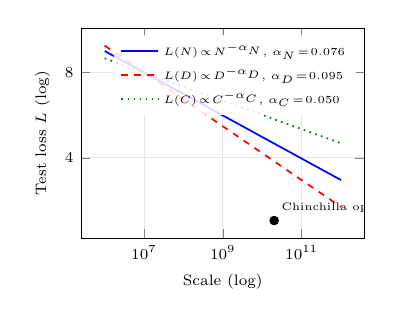
\begin{tikzpicture}[scale=0.78]
\begin{axis}[
  width=6.2cm, height=5cm,
  xmode=log, ymode=log,
  xlabel={Scale (log)},
  ylabel={Test loss $L$ (log)},
  xtick={1e7,1e9,1e11},
  xticklabels={$10^{7}$,$10^{9}$,$10^{11}$},
  ytick={2,4,8},
  yticklabels={2,4,8},
  grid=both,
  grid style={gray!20},
  tick label style={font=\scriptsize},
  label style={font=\scriptsize},
  legend style={font=\tiny, at={(0.97,0.97)}, anchor=north east, draw=none, fill=white, fill opacity=0.85, text opacity=1},
  legend cell align={left},
]
\addplot[blue, thick, domain=1e6:1e12, samples=40] {8 * (1e7/x)^0.076};
\addlegendentry{$L(N)\!\propto\!N^{-\alpha_N}$, $\alpha_N\!=\!0.076$}
\addplot[red, thick, dashed, domain=1e6:1e12, samples=40] {8 * (1e7/x)^0.095};
\addlegendentry{$L(D)\!\propto\!D^{-\alpha_D}$, $\alpha_D\!=\!0.095$}
\addplot[green!50!black, thick, dotted, domain=1e6:1e12, samples=40] {8 * (1e7/x)^0.050};
\addlegendentry{$L(C)\!\propto\!C^{-\alpha_C}$, $\alpha_C\!=\!0.050$}
% Mark a stylized Chinchilla "compute-optimal" point
\addplot[mark=*, only marks, mark size=2pt, mark options={fill=black}] coordinates {(2e10, 2.4)};
\node[font=\tiny, anchor=south west] at (axis cs:2e10, 2.4) {Chinchilla opt.};
\end{axis}
\end{tikzpicture}\\
{\scriptsize Three power-laws on one set of axes: parameters $N$, data $D$, compute $C$. Chinchilla optimum is where the $N$-curve and the $D$-curve cross under a fixed compute budget.}
\end{center}
\end{columns}
\end{frame}

\begin{frame}{Chinchilla (Hoffmann et al.\ 2022): Data $\propto$ Params}
\begin{itemize}
\item Kaplan suggested ``mostly scale parameters.'' Chinchilla revisited the question with a different fitting method and found:
\[
   \text{compute-optimal} \;\Longrightarrow\; D^* \approx 20 \cdot N^*.
\]
For each parameter, you want $\sim$20 training tokens.

\medskip
\item \textbf{Earlier models were undertrained.} GPT-3 (175B params, 300B tokens) used $\sim$$1.7$ tokens/param. A Chinchilla-optimal model at 175B would need $\sim$3.5T tokens.

\medskip
\item \textbf{Chinchilla itself}: 70B params trained on 1.4T tokens --- beat 280B Gopher on most benchmarks.

\medskip
\item \textbf{Modern overtraining:} for inference cost reasons, frontier models now go \emph{past} Chinchilla-optimal --- e.g.\ Llama-3 8B trained on 15T tokens ($\sim$1{,}900 tokens/param). Smaller, more-overtrained model = cheaper to deploy.

\medskip
\item \textbf{The economic frame:} pre-train compute is a one-time fixed cost; inference compute is a recurring marginal cost. Optimal allocation depends on expected serving volume.
\end{itemize}
\end{frame}

\begin{frame}{Emergent Capabilities --- and the ``Mirage'' Critique}
\begin{itemize}
\item \textbf{Wei et al.\ (2022):} on certain tasks (multi-step arithmetic, BIG-Bench, in-context learning), accuracy is near random for small models and then \emph{jumps} sharply at a critical scale.
\item Examples cited: 3-digit addition, word-in-context disambiguation, instruction-following.
\item Coined the term \emph{emergent capabilities}: not present in smaller siblings, suddenly present in larger ones.

\medskip
\item \textbf{Schaeffer, Miranda \& Koyejo (2023, ``Are Emergent Abilities a Mirage?''):}
\begin{itemize}
\item The sharp jumps may be artifacts of \emph{discontinuous metrics} (exact-match accuracy).
\item Switch to a continuous metric (e.g.\ token edit distance, partial credit) and the curves become smooth power-laws.
\item ``Emergence'' may be in our metrics, not in the underlying loss.
\end{itemize}

\medskip
\item \textbf{Where this leaves us:}
\begin{itemize}
\item Capability \emph{does} grow with scale --- empirically robust.
\item Whether it grows ``smoothly'' or ``in jumps'' depends on how you measure.
\item For an economist: \emph{always} look at the loss curve, not just the headline accuracy.
\end{itemize}
\end{itemize}
\end{frame}

%=============================================================================
\section{Synthesis}

\begin{frame}{Transformer vs.\ LDA Topic Models}
\begin{columns}[T]
\column{0.48\textwidth}
\begin{tcolorbox}[colback=blue!5, colframe=blue!50!black, title=\textbf{LDA / topic models}]
\begin{itemize}
\item Document = mixture of latent topics
\item Bag of words: ignores order
\item Output: topic-word and document-topic distributions
\item Strength: interpretable themes
\item Weakness: cannot generate coherent prose
\end{itemize}
\end{tcolorbox}

\column{0.48\textwidth}
\begin{tcolorbox}[colback=green!5, colframe=green!40!black, title=\textbf{Transformers}]
\begin{itemize}
\item Token-by-token, order-aware
\item Captures syntax and long-range dependencies
\item Output: contextual embeddings + a generative model
\item Strength: rich generation, fluent prose, classification
\item Weakness: less directly interpretable
\end{itemize}
\end{tcolorbox}
\end{columns}

\medskip
\textbf{When to use what:} LDA is still excellent for thematic structure and quick descriptive analysis on small corpora. Transformers dominate when you need generation, classification, or context-aware embeddings.
\end{frame}

\begin{frame}[fragile]{Structured Output: JSON as a Measurement Tool}
\small
\begin{columns}[T]
\column{0.50\textwidth}
\textbf{Free-text answers are unstable.} A rubric that asks for ``hawkish / dovish / neutral'' may produce \texttt{Hawkish.}, \texttt{`hawkish'}, \texttt{The label is hawkish.}, or worse. Post-processing such variation is brittle and undermines reproducibility.

\medskip
\textbf{Solution.} Force the model to emit a fixed-schema JSON object. Every provider exposes a ``structured output'' / ``tool use'' API that constrains decoding (logit masking over disallowed tokens) so the output is \emph{guaranteed} to parse.

\medskip
\textbf{Mechanism.} The model is still next-token predicting. The provider's API simply masks tokens that would violate the schema --- the next-token distribution is restricted to syntactically valid continuations.

\medskip
\textbf{Why it bridges to Lec09.} An ``agent'' is just an LLM whose schema names \emph{tools to call}, not labels to output. The same machinery.

\column{0.46\textwidth}
\textbf{Sentiment-extraction schema:}
\begin{lstlisting}[language={},basicstyle=\scriptsize\ttfamily,frame=single,backgroundcolor=\color{gray!8}]
{
  "stance": "hawkish|dovish|neutral",
  "confidence": 0.0,
  "evidence_phrase": ""
}
\end{lstlisting}

\medskip
\textbf{Tool-call schema (Lec09 preview):}
\begin{lstlisting}[language={},basicstyle=\scriptsize\ttfamily,frame=single,backgroundcolor=\color{gray!8}]
{
  "tool": "fred_query",
  "args": {
    "series": "UNRATE",
    "start": "2020-01"
  }
}
\end{lstlisting}

\smallskip
\scriptsize
\textbf{For econ research:} schemas \emph{enforce} the rubric (no off-rubric labels), expose the model's evidence (auditable), and let you compute Cohen's $\kappa$ on parseable output. Every data-extraction pipeline in T4 ships with one.
\end{columns}
\end{frame}

\begin{frame}{Three Ways to Adapt an LLM}
\begin{center}
\renewcommand{\arraystretch}{1.35}
\begin{tabular}{p{3.2cm} p{4.2cm} p{4.5cm}}
\toprule
\textbf{Method} & \textbf{What changes} & \textbf{Best for} \\
\midrule
Prompt engineering & Only the input text & Quick experiments, zero-cost adaptation \\
Fine-tuning (LoRA / DAPT) & Some model weights & New behavior or style on a fixed domain \\
Retrieval-Augmented Generation (RAG) & Relevant external context injected at inference time & New \emph{facts} the model never saw \\
\bottomrule
\end{tabular}
\end{center}

\medskip
\begin{itemize}
\item All three are non-exclusive. In practice you often combine them.
\item RAG addresses the problem we will dwell on at the end of this lecture: \emph{the model's knowledge has a cutoff date}.
\item Lecture 8 is dedicated to RAG.
\end{itemize}
\end{frame}

\begin{frame}{Revisiting: Why One Equation Enables So Much}
\begin{itemize}
\item Now that we understand pretraining, fine-tuning, and generation, the opening claim makes mechanical sense:
\[
   p\bigl(t^{(n+1)} \mid t^{(1)}, \ldots, t^{(n)}\bigr) \quad \text{is all there is.}
\]

\medskip
\item \textbf{Summarizing a 10-K filing:} the prompt carries the document and the instruction; the model predicts summary tokens one by one because pretraining exposed it to millions of (long-document, summary) pairs.

\medskip
\item \textbf{Extracting FOMC stance:} fine-tuning on labeled central bank text shifts the next-token distribution so that stance-label tokens are most probable after a monetary-policy sentence.

\medskip
\item \textbf{Generating scenario forecasts:} condition on macro variables and a scenario description; next-token prediction fills in the narrative consistently with the conditioning.

\medskip
\item \textbf{Writing and debugging code:} the training corpus included billions of code tokens; the objective is identical --- next token, given context.

\medskip
\item \textbf{The unifying insight:} all tasks are the same computation. Pretraining provides the knowledge; prompts and fine-tuning steer \emph{which} next-token distribution we sample from. Every capability is a special case of the one equation.

\medskip
\item \textbf{Bridge to T3b.} The same next-token engine is what \emph{hallucinates}, drifts across versions, and reads ``lost in the middle.'' Topic 7.3b audits these structural limits before we use LLMs as measurement instruments.
\end{itemize}
\end{frame}

\end{document}
